\documentclass{article}

\usepackage[utf8]{inputenc}
\usepackage{amssymb}
\usepackage{amsmath}
\usepackage{float}
\usepackage{latexsym}
\usepackage{subcaption}
\usepackage{gensymb}
\usepackage{caption}
\usepackage{fancyhdr}
\usepackage{lastpage}
\usepackage{extramarks}
\usepackage[usenames,dvipsnames]{color}
\usepackage{graphicx}
\usepackage{listings}
\usepackage{courier}
\usepackage{lipsum}
\usepackage{tabularx}
\usepackage{color}
\usepackage{algorithm}
\usepackage[noend]{algpseudocode}

\definecolor{mygreen}{rgb}{0,0.6,0}
\definecolor{mygray}{rgb}{0.5,0.5,0.5}
\definecolor{mymauve}{rgb}{0.58,0,0.82}

\lstset{
  backgroundcolor=\color{white},   
  breaklines=true,
  captionpos=b,
  commentstyle=\color{mygreen},
  escapeinside={\%*}{*)},
  extendedchars=true,
  frame=single,
  keepspaces=true,
  keywordstyle=\color{blue},
  language=Octave,
  otherkeywords={*,...},
  numbers=left,
  numbersep=5pt,
  numberstyle=\tiny\color{mygray},
  rulecolor=\color{black},
  showspaces=false,
  showstringspaces=false,
  showtabs=false,
  stepnumber=2,
  stringstyle=\color{mymauve},
  tabsize=2,
  title=\lstname
}

\topmargin=-0.45in
\evensidemargin=0in
\oddsidemargin=0in
\textwidth=6.5in
\textheight=9.0in
\headsep=0.25in
\linespread{1.1} % Line spacing

%\lhead{Set Header} % Top left header
\chead{}
\lfoot{\lastxmark} % Bottom left footer
\cfoot{} % Bottom center footer
\rfoot{Page\ \thepage} % Bottom right footer
\renewcommand\headrulewidth{0.4pt} % Size of the header rule
\renewcommand\footrulewidth{0.4pt} % Size of the footer rule
\setlength\parindent{16pt} % Removes all indentation from paragraphs
\setcounter{secnumdepth}{0} % Removes default section numbers
\title{
\vspace{1in}
\textmd{\textbf{Insert Title}} \\
\author{Christoffer Thrysøe - dfv107}
}

\begin{document}
\maketitle
\pagenumbering{arabic}
\section{1. Introduction of New Products}
\subsection*{1.1 Known T}
We have an esablished product on the market, which we know sells with probability $\mu = 0.5$. We also have a new product, which sells with an unknown probability $\mu$. At every sales round, we can only offer one product. We wish to propose a strategy, which maximizes the sales and analyse it's pseudo regret. For this assignment, I assume that we know the time horizon T, beforehand. I also assume that we are in bandit setting, i.e if we should try to sell the established product, where $\mu=0.5$, we do not know if the new product would sell or not. \\
Since we know the time horizon T, we can use the exploration/exploitation approach, where the exploration phase determines the optimal product and the exploitation phase sells the optimal product. Since the sale probability of the established product is known, we only need to explore the new product. If we denote the established product by $a_{old}$ and the new product $a_{new}$.
The algorithm for employing the above strategy can be described as followed:
\begin{algorithm}[H]
\caption{Maximize Sale}
\hspace*{\algorithmicindent}\textbf{Input:} $\text{Time Horizon: } T$ \\
\hspace*{\algorithmicindent}$\text{error}=0$ 
\begin{algorithmic}[1]
%\Procedure{Hedge}{}
\For {$t=1,2, \dots, \epsilon T $ }
\State \text{Sell $A_t = a_{new}$}
\If{$\text{not sale}(A_t)$} \State $\text{error} \pm 1 $
\EndIf
\EndFor
%\State $\text{avg\_error} = \text{error} / \epsilon T$
\State $\text{sale\_prob} =  1 - \left(\text{error} / \epsilon T  \right)$
\State $\Delta = 0.5 - \text{sale\_prob}$
\If{$\Delta < 0$} \State $a_{opt} = a_{new}$
\Else \State $a_{opt} = a_{old}$
\EndIf
\For {$t=\epsilon T+1 , \dots, T$}
\State $\text{Sell } A_t = a_{opt}$
\EndFor
\end{algorithmic}
\end{algorithm}
Where we do $\epsilon T$ iterations of exploration (i.e. try to sell the unknown product) and $(1-\epsilon)T$ iterations of exploitation. The gap $\Delta$ is negative if the estimated sale probability is greater than $0.5$, in which the optimal product is the new product. We wish to maximise the sale of the above algorithm, thus we want to pick $\epsilon$ in such a way that it minimises the regret of the above algorithm. Here I will use the same approach as for the lecture notes, where we define $\delta(\epsilon)$ to be the probability of picking the wrong product to be the most selling one after $\epsilon T$ rounds of exploration. Then we bind the regret as followed:
\begin{equation}
\label{eq:1regret}
\bar{R}_T \leq \dfrac{1}{2} \Delta \epsilon T + \delta(\epsilon) \Delta(1-\epsilon) T \leq \dfrac{1}{2} \Delta \epsilon T + \delta(\epsilon) \Delta T = \left( \dfrac{1}{2} \epsilon + \delta(\epsilon) \right) \Delta T 
\end{equation}
Now we wish to express the probability $\delta(\epsilon)$, which we will do by binding it. We measure the algorithms performance of the exploration phase by $\hat{\mu}_{\epsilon T}(a)$, which is the empirical loss/reward at round $\epsilon T$. We want to pick the product, which resulted in the most optimal empirical loss/reward. Below binds the probability of picking a suboptimal arm after the exploration phase.
\begin{align}
\delta(\epsilon) &= P \lbrace \hat{\mu}_ {\epsilon T}(a) \geq \hat{\mu}_{\epsilon T}(a^*)  \rbrace \\
&\leq P \lbrace \hat{\mu}_{\epsilon T} (a) \geq \mu(a) + \dfrac{1}{2} \rbrace + P \lbrace \hat{\mu}_{\epsilon T}(a^*) \leq \mu^* - \dfrac{1}{2} \Delta \rbrace \\
&\leq 2 e^{ -2 \epsilon T (\frac{1}{2} \Delta)^2} = 2 e ^{ -\epsilon T \Delta^2 / 2 }
\label{eq:1}
\end{align}
where the last line follows from Hoeffding's inequality. Note that since we are exploring the unknown product at each sales round, we get full information as we know the sales probability of the existing product. That is why we don't divide by two in \eqref{eq:1}. Now that we have a bound for $\delta(\epsilon)$ we can use this in \eqref{eq:1regret}, resulting in the following:
\begin{equation}
\label{eq:1reg1}
\bar{R}_T \leq \left( \dfrac{1}{2} \epsilon + 2 e ^{ -\epsilon T \Delta^2 / 2 } \right) \Delta T
\end{equation}
To minimize \eqref{eq:1reg1}, we want the two sums to contribute equally, thus we have that $\epsilon = 4 e ^{ -\epsilon T \Delta^2 / 2 }$, which leads to the approximation of $\epsilon$: $\epsilon \approx \dfrac{\text{ln}(2T \Delta^2 )}{T \Delta^2 / 2}$
Thus we get the following bound on the regret:
\begin{align}
\bar{R}_T &\leq \dfrac{1}{2} \dfrac{\text{ln}(2T \Delta^2 )}{T \Delta^2 / 2} + 2 e^{ - \left(\frac{\text{ln}(2T \Delta^2 ) T}{T \Delta^2 / 2} \right) T \Delta^2 / 2 } \Delta T \\
&= \dfrac{\text{ln}(2T \Delta^2 )}{T \Delta^2} + 2 e^{ - \text{ln}(2T \Delta^2 )  } \Delta T \\
&=  \dfrac{\text{ln}(2T\Delta^2)}{\Delta} + \dfrac{1}{\Delta} 
\end{align}
Therefore the regret of the approach can be bounded by:
\begin{equation}
\bar{R}_T \leq \dfrac{\text{ln}(2T\Delta^2)}{\Delta} + \dfrac{1}{\Delta} 
\end{equation}
The optimal number of explorations rounds, which minimizes the pseudo regret is given by: 
\begin{equation}
\label{eq:opteps}
\epsilon T = \dfrac{\text{ln}(2T \Delta^2 )}{T \Delta^2 / 2}
\end{equation}
Thus the previous proposed algorithm, from this task, can be altered to use the $\epsilon$ from \eqref{eq:opteps}, which minimizes the pseudo regret. 
\subsection{1.2 Unknown T}
If the time horizon T is unknown, we cannot do an exploration phase, as we will not know the optimal length of this time period. If we instead do an approach similar to "Follow the leader", we can choose the most successful product at each $t$ and since we know the $\mu(a_{old})$ of the existing product, we only need to check if $\hat{\mu}(a_{new})$ is greater than $0.5$. The issue is, however that since we are in bandit setting, if we pick the existing product, we will have no way of estimating the sale probability of the new product. For example if the unknown product has a bad start, we will only pick the existing product, leaving an uncertainty of the new product. Thus we wish to add a reward/upside to picking the arm if we are uncertain about the true sales probability. This is done by the \texttt{UCB1} algorithm, which takes an upper confidence bound $U_t(a)$ on $\mu(a)$:
\begin{equation}
U_t(a) = \hat{\mu}_{t-1}(a) + \sqrt{\dfrac{3 \text{ ln } t}{2 N_{t-1}(a)}}
\end{equation}
where $N_{t-1}(a)$ is the number of times the arm $a$ has been pulled. Thus the added term increases when the arm is unexplored and decreases if the arm is explored. This added term will help us explore the unknown product, so that we get a correct estimate 

%TODO write up new approach depending on epsilon
\section{2. Tighter analysis of the Hedge algorithm}
We wish to bind the following, using Hoeffding's lemma: 
\begin{equation}
\label{eq:21}
\sum\limits_{a} e^{-\eta X_t^a} p_t(a)  
\end{equation}
Hoeffding's lemma is defined as:
\begin{equation}
\mathbb{E}[e^{\lambda X}] \leq e^{\lambda \mathbb{E}[X] + \frac{\lambda^2(b-a)^2}{8}}
\end{equation}
where $b$ is the largest value $X_t$ can take, and $a$ is the smallest value $X_t$ can take. First we note that \eqref{eq:21} is the same as the expected value of $e^{-\eta X_t^ a}$ with respect to the distribution $p_t$, thus we can write:
\begin{equation}
\label{eq:22}
\sum\limits_{a} e^{-\eta X_t^a} p_t(a) = \mathbb{E}_{p_t}[e^{-\eta X_t^a}]
\end{equation}
Applying hoeffding's lemma to the right hand side of \eqref{eq:22}, we get the following:
\begin{align}
\mathbb{E}_{p_t}[e^{-\eta X_t^a}] &\leq e^{-\eta \mathbb{E}_{p_t}[X_t^a] + \frac{\eta^2 (\text{max}(X_t) - \text{min}(X_t))^2}{8} } \\
&= e^{- \eta \sum\limits_{a} X_t^a p_t(a) + \frac{\eta^2 (\text{max}(X_t) - \text{min}(X_t))^2}{8} }
\label{eq:23}
\end{align}
where \eqref{eq:23} follows from writing out the expected value. \\
We now continue the proof from the lecture notes, where we defined $W_t = \sum_a e^{-\eta L_t(a)}$, where $L_t(a)$ is the accumulated loss for arm $a$ at time $t$.\\
We now have the ratio, which we must sum for each $t$:
\begin{equation}
\dfrac{W_T}{W_0} \leq e^{- \eta \sum_{t=1}^T \sum_{a} X_t^a p_t(a) + \frac{\eta^2}{8} \sum_{t=1}^T (\text{max}(X_t) - \text{min}(X_t))^2}
\end{equation}
If we assume that the losses $X^t_a$ can take values in the interval $[0,1]$ we have the following:
\begin{equation}
\label{eq:25}
\dfrac{W_T}{W_0} \leq e^{- \eta \sum_{t=1}^T \sum_{a} X_t^a p_t(a) + \frac{\eta^2}{8} \sum_{t=1}^T 1}
\end{equation}
From the lecture notes we have that: 
\begin{equation}
\label{eq:24}
\dfrac{W_T}{W_0} = \dfrac{\sum\limits_a e^{-\eta L_T(a)}}{K} \geq \dfrac{\max_{a}e^{-\eta L_T(a)}}{K} = \dfrac{e^{-\eta \min_a L_T(a)}}{K}
\end{equation}
Combining the inequalities in \eqref{eq:25} and \eqref{eq:24} and taking the logarithm on both sides, we get: 
\begin{equation}
\label{eq:26}
-\eta \min_a L_T(a) - \text{ ln } K \leq - \eta \sum\limits_{t=1}^T \sum\limits_{a} X_t^ a p_t(a) + \dfrac{\eta^2}{8} \sum\limits_{t=1}^T 1
\end{equation}
Rearranging \eqref{eq:26} and dividing by $\eta$ we get the following:
\begin{equation}
\sum\limits_{t=1}^T \sum\limits_a X_t^a p_t(a) - \min_{a} L_T(a) \leq \dfrac{\text{ ln }k}{\eta} + \dfrac{\eta}{8} \sum\limits_{t=1}^T 1
\end{equation}
We note that the term $\sum_{t=1}^T \sum_{a=1}^K p_t(a) X_t^a$ is the expected cumulative loss of the hedge after $T$ rounds. Subtracting this with the minimum loss, we get the expected regret of the Hedge. Thus we can write: 
\begin{equation}
\label{eq:27}
\mathbb{E}[R_T] \leq \dfrac{\text{ln }K}{\eta}+ \dfrac{\eta}{8}T
\end{equation}
where $T$ follows from summing 1 $T$ times. Now we wish to determine what $\eta$ minimizes the expected regret. To do so, we take the derivative of \eqref{eq:27}, with respect to $\eta$ and set it to zero:
\begin{equation}
\dfrac{\partial}{\partial \eta} \left[ \dfrac{\text{ln }k}{\eta}+ \dfrac{\eta}{8}T \right] = -\dfrac{\text{ln }K}{\eta^2} + \dfrac{T}{8}
\end{equation}
setting it to zero and solving for $\eta$:
\begin{align}
0 &= -\dfrac{\text{ ln }K}{\eta^2} + \dfrac{T}{8} \Rightarrow \\
\eta &= \sqrt{\dfrac{8 \text{ ln }K}{T}}
\end{align}
Now we can plug this value back into the bound on the expected regret in \eqref{eq:27} and get the following:
\begin{align}
\mathbb{E}[R_T] &\leq \dfrac{\text{ln }K}{\eta}+ \dfrac{\eta}{8}T \\
&= \dfrac{\text{ln }K}{\sqrt{\frac{8 \text{ln }K}{T}}}
 + \dfrac{\sqrt{\frac{8 \text{ln }K}{T}}}{8}T \\
&= \dfrac{ \sqrt{T} \sqrt{\text{ln } K }  }{ \sqrt{2}} \\
&= \sqrt{\frac{1}{2} T \text{ ln } K}
\end{align}
Which is what we wanted to prove. Thus, using Hoeffding's lemma, we get
\begin{equation}
\mathbb{E}[R_T] \leq \sqrt{\frac{1}{2} T \text{ ln } K}
\end{equation}
instead of:
\begin{equation}
\mathbb{E}[R_T] \leq \sqrt{2 T \text{ ln } K}
\end{equation}
\section{3. Empirical comparison of FTL and Hedge}
\subsection{1}
We wish to compare the empirical performance of the "Follow the Leader" algorithm with the hedge algorithm, using various learning rates. Their performance will be tested on predicting a binary sequence $X_1,X_2,...$, that is, at each round the algorithm can predict a 0 or 1. The algorithms do not know the bias of the sequence $\mu$, which the sequences are generated with respect to. \\ First I will discuss how the sequence is generated, then I will comment on the algorithms and last compare their performance. \\
For each experiment, we are given a bias $\mu$. At each iteration, a random number $r \in [0,1]$ is drawn and the i'th element of the sequence is sampled as followed:
\begin{equation}
X_i = \begin{cases}
0 &\text{if $\mu < r$}\\
1 &\text{if $\mu \geq r$}
\end{cases}
\end{equation}
Thus at each element in the sequence, we have the probability:
\begin{align}
P\lbrace X_i &= 1 \rbrace = \mu \\
P\lbrace X_i &= 0 \rbrace = 1-\mu
\end{align}
The "Follow the Leader" algorithm picks at round $t$, the arm with the best empirical performance over the previous $t-1$ pulls. The algorithm is defined as followed:
\begin{algorithm}[H]
\caption{Follow The Leader}\label{euclid}
\begin{algorithmic}[1]
\Procedure{FTL}{}
\For {$t=1,2,... do$}
\State $\text{Play } A_t = \text{arg} \max_{a} \hat{\mu}_{t-1}(a)$
\EndFor
\EndProcedure
\end{algorithmic}
\end{algorithm}
The Hedge algorithm is defined as followed:
\begin{algorithm}[H]
\caption{Hedge}
\hspace*{\algorithmicindent}\textbf{Input:} Learning rates $\eta_i \geq 
\eta_2 .... > 0$ \\
\hspace*{\algorithmicindent}$\forall a : L_0(a) = 0$ 
\begin{algorithmic}[1]
%\Procedure{Hedge}{}
\For {$t=1,2,... do$}
\State $\forall a : p_t(a) = \frac{e^{-\eta L_{t-1}(a)}}{\sum_a e^-{\eta L_{t-1}(a)}}$
\State \text{Sample $A_t$ according to $p_t$ and play it}
\State \text{Observe $l_t^1,...,l_t^K$ and suffer $l_t^{A_t}$} 
\State $\forall a: L_t(a) = L_{t-1}(a)+l_t^a$
\EndFor
%\EndProcedure
\end{algorithmic}
\end{algorithm}
Where $L_{t-1}(a)$ is the accumulated loss, until round $t$.
The prediction of the Hedge algorithm is done as followed, $r \in [0,1]$ is picked randomly:
\begin{equation}
X_i = \begin{cases}
0 &\text{if $r < p_t(a_0)$}\\
1 &\text{else}
\end{cases}
\end{equation}
The experiment is performed with the following learning rates for the hedge algorithm:
\begin{equation}
\eta = \sqrt{\dfrac{2 \text{ ln } K}{T}}, \hspace{0.2cm} \eta = \sqrt{\dfrac{8 \text{ ln } K}{T}}, \hspace{0.2cm} \eta_t = \sqrt{\dfrac{\text{ln }K}{t}}, \hspace{0.2cm} \eta_t = 2\sqrt{\dfrac{\text{ln }K}{t}}
\end{equation}
where $T$ is the time horizon, and $t$ is the given time index. Thus the two first weights are constant. The tested values of $\mu$ are the following:
\begin{equation}
\label{eq:mulist}
\mu = \dfrac{1}{2} - \dfrac{1}{4}, \hspace{0.2cm} \mu = \dfrac{1}{2} - \dfrac{1}{8}, \hspace{0.2cm} \mu = \dfrac{1}{2} - \dfrac{1}{16}
\end{equation}
The performance of the algorithms is given by the pseudo regret, which is defined as:
\begin{equation}
\label{eq:pseudo}
\bar{R}_T = \mathbb{E}\left[  \sum\limits_{t=1}^T l_t^{A_t} \right] - T \min_{a} \mu(a)
\end{equation}
We now run the five algorithms (FTL and four variations of the Hedge algorithm), in which we will get a series of predictions. At each time $t$, we know $\mu$ of the optimal and suboptimal arm. To get the expected value of \eqref{eq:pseudo} we simply sum up the $\mu$ for each prediction of either 0 or 1, that is either $\mu$ or $1-\mu$. The experiment is performed for each $\mu$ in \eqref{eq:mulist}, the average pseudo regret over 10 runs and the average pseudo regret + the standard deviation is plotted.
\subsection{Results:}
The following plots of the pseudo regret and the pseudo regret + standard deviations are shown for the three different settings of $\mu$. The scribbled lines shows the average pseudo regret + the standard deviation for each t. The color of the scribbled lines identify what algorithm they are plotted for. The results will be commented and discussed in the next section.\\ \\
$\mathbf{\mu = \dfrac{1}{2} - \dfrac{1}{4}} $:
\begin{figure}[H]
 \centering
  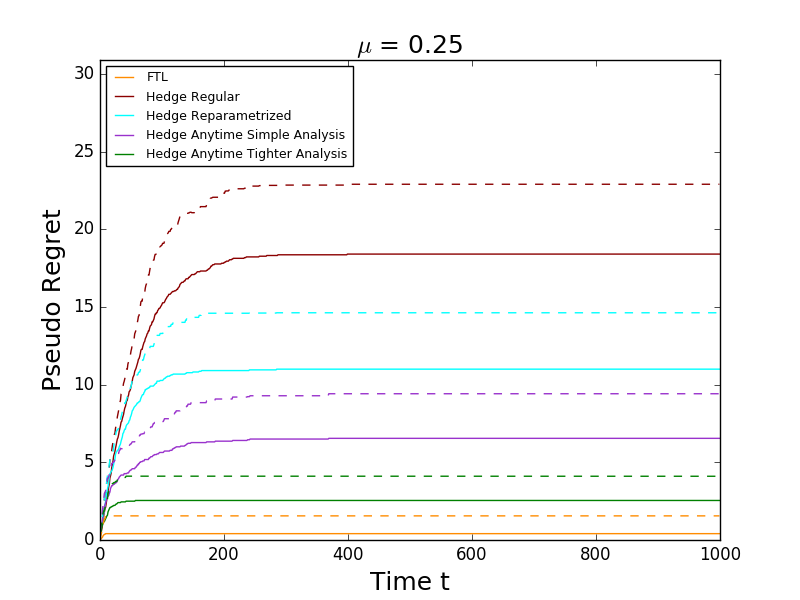
\includegraphics[width=17cm]{fig/0_new.png}
  \caption{\footnotesize Average pseudo regret and average pseudo regret + standard deviation (scribbled line) over 10 runs with $\mu = 0.25$ }
\label{fig:1}
\end{figure}
$\mathbf{\mu = \dfrac{1}{2} - \dfrac{1}{8}} $:
\begin{figure}[H]
 \centering
  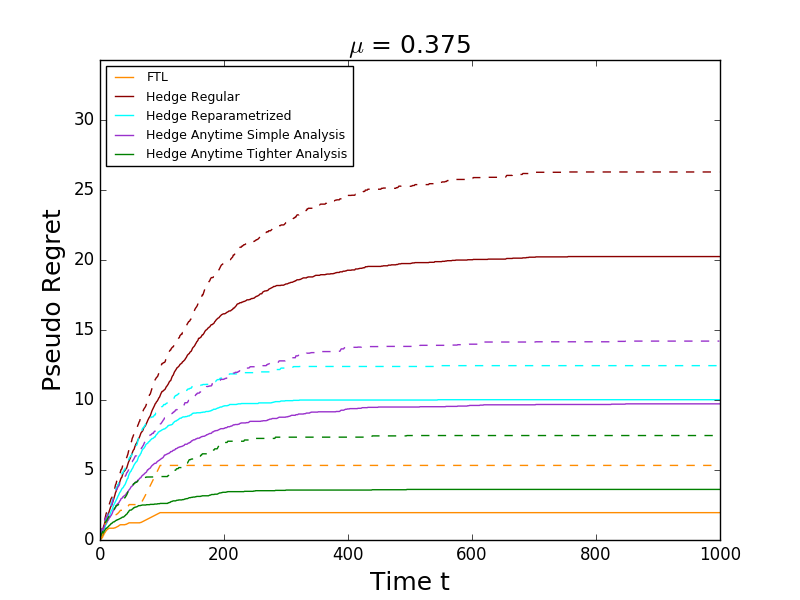
\includegraphics[width=17cm]{fig/1_new.png}
  \caption{\footnotesize Average pseudo regret and average pseudo regret + standard deviation (scribbled line) over 10 runs with $\mu = 0.375$ }
\label{fig:2}
\end{figure}
$\mathbf{\mu = \dfrac{1}{2} - \dfrac{1}{16}} $:
\begin{figure}[H]
 \centering
  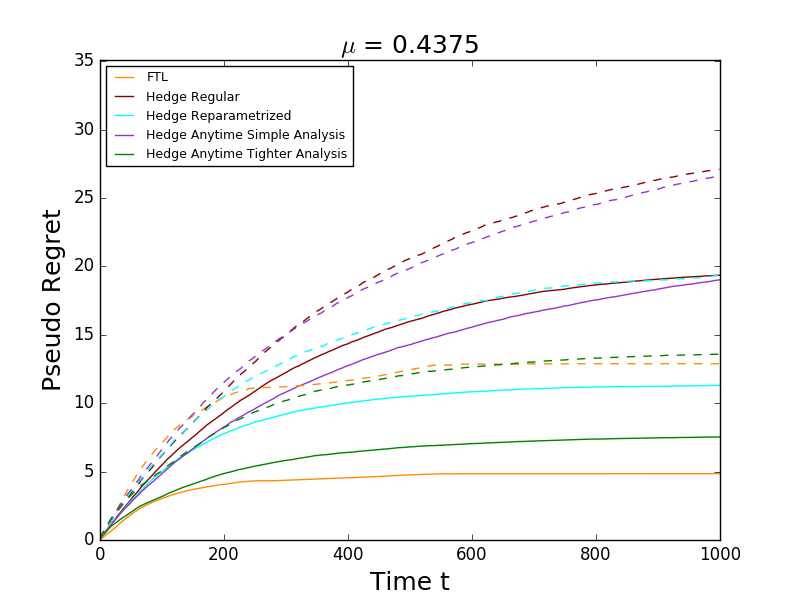
\includegraphics[width=17cm]{fig/2_new.png}
  \caption{\footnotesize Average pseudo regret and average pseudo regret + standard deviation (scribbled line) over 10 runs with $\mu = 0.4375$ }
\label{fig:3}
\end{figure}
\subsection{2}
The "Follow the leader" algorithm has a low pseudo regret compared to the other algorithms. This is because in the pseudo regret, the series of pulled arms is compared to pulling the most optimal arm throughout the experiment. When the bias is low (i.e. the probability is great for one arm and small for the other), the optimal arm will quickly be identified and the "Follow the Leader" algorithm will pull the same arm throughout the experiment. Because it will pull the same arm as the optimal one, the pseudo regret will be low. As evident from figure \ref{fig:1}, the pseudo regret is very low for the FTL approach. There is a small increase in the pseudo regret for the first couple of iterations and then the pseudo regret flattens out. This is because the approach will change between the two arms before identifying the most optimal one. As $t$ increases, the output of the experiment will go towards the true $\mu$, which is why the pseudo regret flattens out. As $\mu$ increases, the optimal arm will be harder to identify, because the gap between the two arms is smaller. This is evident from figure \ref{fig:2}, where the approach takes a longer time identifying the most optimal arm, and \ref{fig:3} where it takes even longer time before identifying the optimal arm. Interestingly the hedge algorithm appears to be more invariant to the increase in $\mu$. Notably the Hedge Anytime with tighter analysis has the best performance, where the Hedge Anytime with simple analysis gets worse as $\mu$ increases. The Hedge with fixed weights $\eta$ performs invariant to the change in $\mu$.
\subsection{3}
For this task, we wish to create a sequence, such that the "Follow the Leader" approach has a bad performance on the sequence. The performance will then be compared to the various versions of the Hedge algorithm. The performance of each algorithm will be measured in regret, which is defined as:
\begin{equation}
R_T = \sum\limits_{t=1}^T l_t^{A_t} - \min_{a} \sum\limits_{t=1}^T l_t^{a}
\end{equation}
thus the performance is measured by the accumulated loss of each pulled arm by the given algorithm, minus the accumulated loss of the arm which resulted in the lowest error in hindsight. The error is the zero-one loss, which is one if the wrong arm is predicted and zero otherwise. The adversarial sequence to the FTL algorithm is simply a sequence, which interchanging picks 0 and 1. This sequence has been chosen because the leader will shift at each iteration. For example if we consider the following sequence, and we take that ties are chosen to be 1:
$$
0,1,0,1,0,1,0,1,0
$$
then the FTL approach will predict the following sequence:
$$
1,0,1,0,1,0,1,0,1
$$
Thus the FTL algorithm will predict wrong at each iteration, whereas the optimal arm only will be wrong half of the iterations. The performance on the adversarial sequence is shown in figure \ref{fig:4} for the five algorithms. The regret is plotted on a log scale, to show the difference between the methods.
\begin{figure}[H]
 \centering
  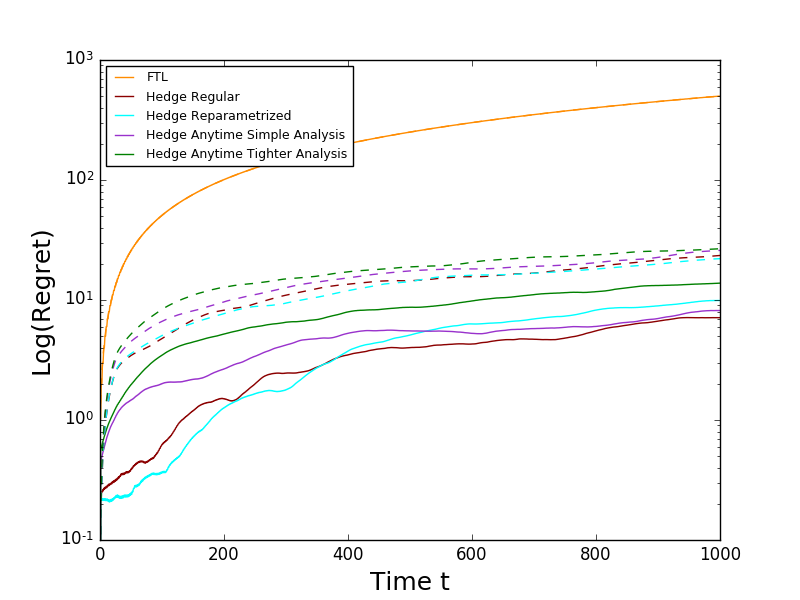
\includegraphics[width=17cm]{fig/adv.png}
  \caption{\footnotesize Average pseudo regret and average pseudo regret + standard deviation (scribbled line) over 10 runs with the adversarial sequence plotted on a log scale to show the difference }
\label{fig:4}
\end{figure}
As evident from figure \ref{fig:4}, the regret of the FTL algorithm is high, whereas the regret for the different variations of the hedge algorithm are low. The regret of the Hedge algorithms are magnitudes lower than the FTL, although fluctuating. It is difficult to identify which algorithm did the best job of predicting the adversarial sequence, but it appears that the Hedge algorithms with fixed weights performed slightly better. But in conclusion the Hedge algorithm performed much better than FTL on the adversarial sequence.

\end{document}
